\documentclass{article}
\usepackage{graphicx}
\begin{document}
\hfill Alejandro Chavez

\hfill Lab 3 - Digital Logic

\hfill \today\\

\begin{center}\begin{large}Lab 3\end{large}\end{center}\begin{itemize}
	\item
		Decoders
	\begin{itemize}
		\item
			Octal Decoder, per textbook.\\
      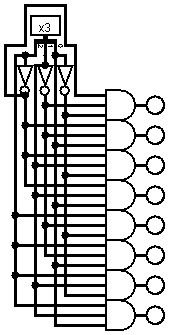
\includegraphics[scale=0.5]{lab3decoder1.png}
		\item
			Octal Decoder, Logisim component.\\
      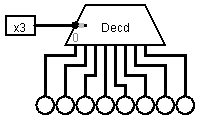
\includegraphics[scale=0.5]{lab3decoder2.png}
	\end{itemize}
	\item
		Multiplexers
	\begin{itemize}
		\item
			2:1 4-bit wide Multiplexer, per textbook.\\
      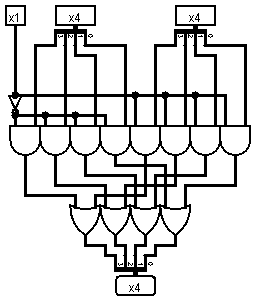
\includegraphics[scale=0.5]{lab3multiplexer1.png}
		\item
			2:1 4-bit wide Multiplexer, Logisim component.\\
      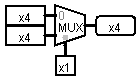
\includegraphics[scale=0.5]{lab3multiplexer2.png}
	\end{itemize}
	\item
		Tiny Alu Circuit
	\begin{itemize}
		\item
			4-bit wide Tiny Alu component.\\
      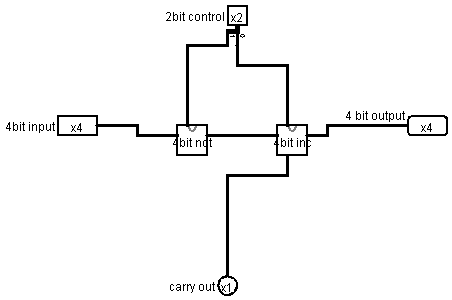
\includegraphics[scale=0.5]{tinyalu.png}
		\item
			Function table for Tiny Alu component\\

      \begin{tabular}{cc|c}
        $A$ & $Op$ & $Out$ \\ \hline
        $k$ & $00$ & $k$\\
        $k$ & $01$ & $if\:k\ge 0, k+1; else\:k-1$\\
        $k$ & $10$ & $if\:k\ge 0, k-7, else\:k+8$\\
        $k$ & $11$ & $if\:k = -1, -1; if\:k>0, k-9; if\:k<-1, k+9$\\
        
      \end{tabular}
	\end{itemize}
\end{itemize}
\end{document}
